% Paquets généraux
\documentclass[a4paper,12pt,titlepage]{article}
\usepackage[T1]{fontenc}
\usepackage[utf8]{inputenc}
\usepackage[french]{babel}
\usepackage[gen]{eurosym}
%\usepackage[dvips]{graphicx}
\usepackage{fancyhdr}
\usepackage{pdfpages} 
\usepackage{multido}
\usepackage{hyperref}
%\usepackage{textcomp}
%\usepackage{aeguill}
\usepackage{schemabloc}
\usepackage[bitstream-charter]{mathdesign}

\newcommand{\id}{54}
\newcommand{\nom}{Liaisons mécaniques}
\newcommand{\sequence}{04}
\newcommand{\num}{01}
\newcommand{\type}{TP}
\newcommand{\descrip}{Modélisation d'un solide. Comportement des liaisons mécaniques. Modéliser les mécanismes du laboratoire par un schéma cinématique, paramétré.}
\newcommand{\competences}{A3-C4: Analyse d'architecture et de comportement \\ &  Mod1-C1: Isolement d'un solide ou d'un système de solides \\ &  Mod2-C10-1: Modèle de solide indéformable \\ &  Mod2-C11: Modélisation géométrique et cinématique des mouvements entre solides indéformables \\ &  Mod2-C12: Modélisation cinématique des liaisons entre solides \\ &  Mod2-C15: Modélisation des actions mécaniques \\ &  Rés-C6: Utilisation d'un solveur ou d'un logiciel multi physique \\ &  Com1-C1: Différents descripteurs introduits dans le programme \\ &  Com2-C4: Outils de communication}
\newcommand{\nbcomp}{9}
\newcommand{\systemes}{Plateforme Stewart}
\newcommand{\systemessansaccent}{Plateforme Stewart}
\newcommand{\ilot}{2}
\newcommand{\ilotstr}{02}
\newcommand{\dossierilot}{\detokenize{Ilot_02 Plateforme Stewart}}
\newcommand{\imageun}{Plateforme}

\newcommand{\urlsysteme}{\href{https://www.costadoat.fr/systeme/57}{Ressources système}}
\newcommand{\matlabsimscape}{\href{https://github.com/Costadoat/Sciences-Ingenieur/raw/master/Systemes/Plateforme Stewart/Plateforme_Stewart_Simscape.zip}{Modèle Simscape}}
\newcommand{\solidworks}{\href{https://github.com/Costadoat/Sciences-Ingenieur/raw/master/Systemes/Plateforme Stewart/Plateforme_Stewart_Solidworks.zip}{Modèle Solidworks}}
\newcommand{\edrawings}{\href{https://github.com/Costadoat/Sciences-Ingenieur/raw/master/Systemes/Plateforme Stewart/Plateforme_Stewart.EASM}{Modèle eDrawings}}
\newcommand{\test}{Stewart_param1}
\newcommand{\testi}{Stewart_param2}
\newcommand{\testii}{Stewart_param3}
\newcommand{\testiii}{Stewart_param4}
\newcommand{\testiiii}{Stewart_euler}

\newcommand{\auteurun}{Renaud Costadoat}
\newcommand{\auteurdeux}{Françoise Puig}
\newcommand{\institute}{Lycée Dorian}


\usepackage{color}
\usepackage{xcolor}
\usepackage{colortbl}
\usepackage{helvet}
\renewcommand{\familydefault}{\sfdefault}
\usepackage{amsfonts}
\usepackage{amsmath}
%\usepackage{xspace}
\usepackage{varioref}
\usepackage{tabularx}
%\usepackage{floatflt}
\usepackage{graphics}
\usepackage{wrapfig}
\usepackage{textcomp}
\usepackage{tikz}
\usepackage{wrapfig}
\usepackage{gensymb}
\usepackage[european]{circuitikz}
\usetikzlibrary{babel}
\usepackage{ifthen}
\usepackage{cancel}
\usepackage{etoolbox}
\usepackage{multirow}
%\usepackage{boxedminipage}
\definecolor{gris25}{gray}{0.75}
\definecolor{bleu}{RGB}{18,33,98}
\definecolor{bleuf}{RGB}{42,94,171}
\definecolor{bleuc}{RGB}{231,239,247}
\definecolor{rougef}{RGB}{185,18,27}
\definecolor{rougec}{RGB}{255,188,204}%255,230,231
\definecolor{vertf}{RGB}{103,126,82}
\definecolor{vertc}{RGB}{220,255,191}
\definecolor{forestgreen}{rgb}{0.13,0.54,0.13}
\definecolor{blcr}{rgb}{0.59,0.69,0.84}
\definecolor{blfr}{rgb}{0.32,0.51,0.75}
\definecolor{orfr}{rgb}{0.90,0.42,0.15}
\definecolor{orcr}{rgb}{0.90,0.65,0.50}
\definecolor{orangef}{rgb}{0.659,0.269,0.072}
\definecolor{orange}{rgb}{0.58,0.35,0.063}
\definecolor{orangec}{rgb}{0.43,0.32,0.25}
\definecolor{rcorrect}{rgb}{0.6,0,0}
\definecolor{sequence}{rgb}{0.75,0.75,0.75}
\definecolor{competences}{rgb}{0.61,0.73,0.35}
\definecolor{grisf}{HTML}{222222}
\definecolor{grisc}{HTML}{636363}
\definecolor{normal}{HTML}{4087c4}
\definecolor{info}{HTML}{5bc0de}
\definecolor{success}{RGB}{92,184,92}
\definecolor{warning}{RGB}{240,173,78}
\definecolor{danger}{RGB}{217,83,79}
\hypersetup{                    % parametrage des hyperliens
    colorlinks=true,                % colorise les liens
    breaklinks=true,                % permet les retours à la ligne pour les liens trop longs
    urlcolor= blfr,                 % couleur des hyperliens
    linkcolor= orange,                % couleur des liens internes aux documents (index, figures, tableaux, equations,...)
    citecolor= forestgreen                % couleur des liens vers les references bibliographiques
    }

% Mise en page
\pagestyle{fancy}

\setlength{\hoffset}{-18pt}

\setlength{\oddsidemargin}{0pt} 	% Marge gauche sur pages impaires
\setlength{\evensidemargin}{0pt} 	% Marge gauche sur pages paires
\setlength{\marginparwidth}{00pt} 	% Largeur de note dans la marge
\setlength{\headwidth}{481pt} 	 	% Largeur de la zone de tête (17cm)
\setlength{\textwidth}{481pt} 	 	% Largeur de la zone de texte (17cm)
\setlength{\voffset}{-18pt} 		% Bon pour DOS
\setlength{\marginparsep}{7pt}	 	% Séparation de la marge
\setlength{\topmargin}{-30pt} 		% Pas de marge en haut
\setlength{\headheight}{35pt} 		% Haut de page
\setlength{\headsep}{20pt} 		% Entre le haut de page et le texte
\setlength{\footskip}{30pt} 		% Bas de page + séparation
\setlength{\textheight}{700pt} 		% Hauteur de l'icone zone de texte (25cm)
\setlength\fboxrule{1 pt}
\renewcommand{\baselinestretch}{1}
\setcounter{tocdepth}{1}
\newcommand{\cadre}[2]
{\fbox{
  \begin{minipage}{#1\linewidth}
   \begin{center}
    #2\\
   \end{center}
  \end{minipage}
 }
}

\newcounter{num_quest} \setcounter{num_quest}{0}
\newcounter{num_rep} \setcounter{num_rep}{0}
\newcounter{num_cor} \setcounter{num_cor}{0}

\newcommand{\question}[1]{\refstepcounter{num_quest}\par
~\ \\ \parbox[t][][t]{0.15\linewidth}{\textbf{Question \arabic{num_quest}}}\parbox[t][][t]{0.93\linewidth}{#1}\par
}


\newcommand{\reponse}[1]
{\refstepcounter{num_rep}
\noindent
\rule{\linewidth}{.5pt}
\textbf{Question \arabic{num_rep}:}
\multido{\i=1+1}{#1}{~\ \\}
}

\newcommand{\cor}
{\refstepcounter{num_cor}
\noindent
\rule{\linewidth}{.5pt}
\textbf{Question \arabic{num_cor}:} \\
}

\newcommand{\titre}[1]
{\begin{center}
\cadre{0.8}{\huge #1} 
\end{center}
}


% En tête et pied de page
\fancypagestyle{normal}{%
  \fancyhf{}
\lhead{\nom}
\rhead{
\includegraphics[width=2cm]{../../img/logo}\hspace{2pt}}
\ifdef{\auteurdeux}{\lfoot{\auteurun,\auteurdeux}}{\lfoot{\auteurun}}
\cfoot{Page \thepage}}

\fancypagestyle{correction}{%
  \fancyhf{}
  \lhead{\colorbox{danger}{\begin{minipage}{0.65\paperwidth} \textcolor{white}{\textbf{Correction}} \end{minipage}} }
  \rhead{
\includegraphics[width=2cm]{../../img/logo}}
  \ifdef{\auteurdeux}{\lfoot{\auteurun,\auteurdeux}}{\lfoot{\auteurun}}
  \rfoot{\colorbox{danger}{\begin{minipage}{0.5\paperwidth} \begin{flushright}\textcolor{white}{\textbf{Correction}}\end{flushright} \end{minipage}} }}

\renewcommand{\footrulewidth}{0.4pt}

\usepackage{eso-pic}
\newcommand{\BackgroundPic}{%
\put(0,0){%
\parbox[b][\paperheight]{\paperwidth}{%
\vfill
\begin{center}
\hspace{0.5cm}\vspace{0.5cm}
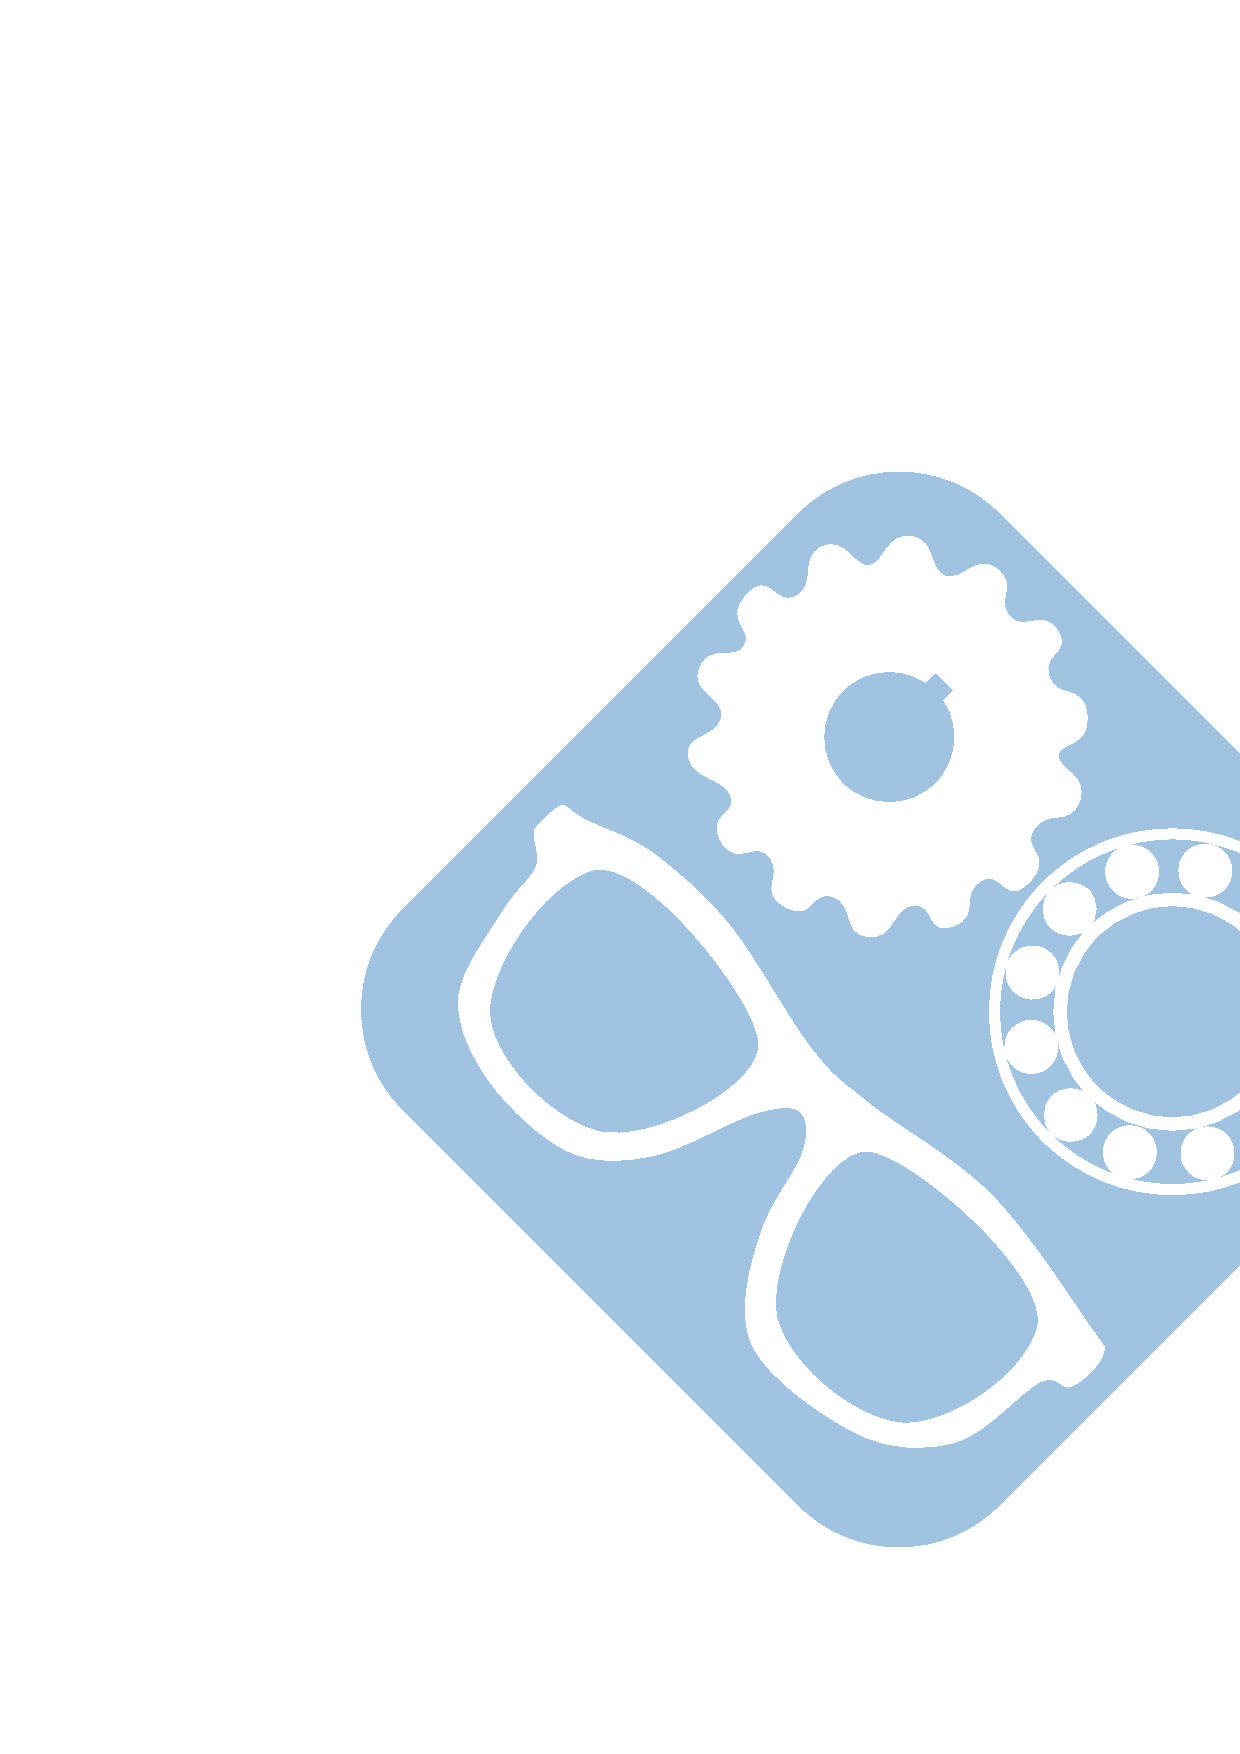
\includegraphics[width=\paperwidth,height=\paperheight,%
keepaspectratio]{../../img/fond3}%
\end{center}
\vfill
}}}

\newcommand{\BackgroundPicdeux}{%
\put(25,-30){%
\parbox[b][\paperheight]{\paperwidth}{%
\vfill
\begin{center}
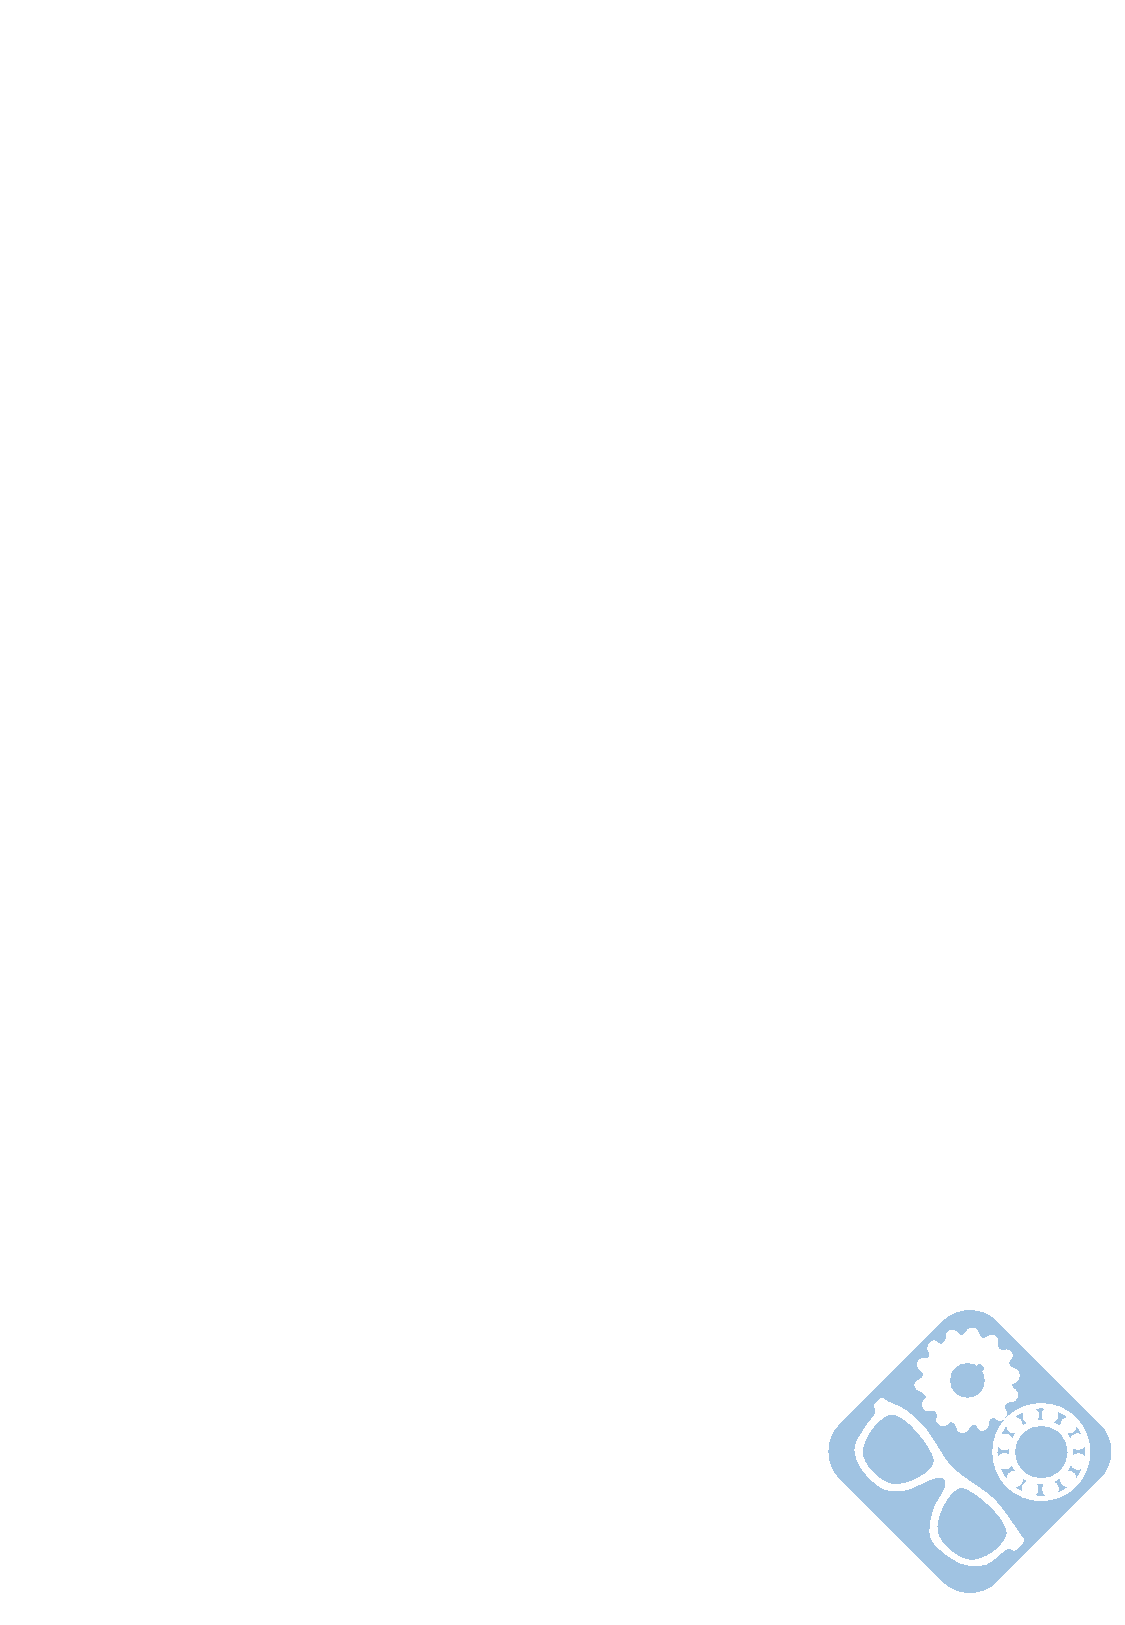
\includegraphics[width=\paperwidth,height=\paperheight,%
keepaspectratio]{../../img/fond4}%
\end{center}
\vfill
}}}

\begin{document}

\pagestyle{empty}

\vspace*{-3\baselineskip}

\AddToShipoutPicture*{\BackgroundPic}

\ifdef{\auteurdeux}{\begin{tabular}{>{\columncolor{gray!00}}m{.3\linewidth} m{.3\linewidth} >{\columncolor{gray!00}}m{.3\linewidth}}
Séquence : \sequence &  \multirow{3}{*}{\hspace{1cm}
\includegraphics[height=1.5cm]{../../img/logo}} &  \begin{flushright} \multirow{4}{*}{\hspace{1cm}
\includegraphics[height=4cm]{img/qrcode}}\end{flushright}\\
Document : \type\num \\
 \institute \\
 \auteurun\\
 \auteurdeux
\end{tabular}}{\begin{tabular}{>{\columncolor{gray!00}}m{.3\linewidth} m{.3\linewidth} >{\columncolor{gray!00}}m{.3\linewidth}}
Séquence : \sequence &  \multirow{3}{*}{\hspace{1cm}
\includegraphics[height=1.5cm]{../../img/logo}} &  \begin{flushright} \multirow{4}{*}{\hspace{1cm}
\includegraphics[height=4cm]{img/qrcode}}\end{flushright}\\
Document : \type\num \\
 \institute \\
 \auteurun
\end{tabular}}

\vspace{1cm}

\ifdef{\prive}{\begin{center}\colorbox{danger}{\Huge{Avec Correction}}\end{center}}{}

\begin{center}\huge{\nom}\end{center}

\vspace{2cm}

\ifdef{\imagedeux}{\begin{minipage}{0.49\linewidth}}{}
\begin{center}\includegraphics[height=5cm]{/home/renaud/Documents/Renaud/GitHub/django_education/systemes/\imageun}\end{center}
\ifdef{\imagedeux}{\end{minipage}\hfill
\begin{minipage}{0.49\linewidth}
\begin{center}\includegraphics[height=5cm]{/home/renaud/Documents/Renaud/GitHub/django_education/systemes/\imagedeux}\end{center}
\end{minipage}}{}

\vspace{5cm}


\begin{tabular}{p{.15\linewidth} >{\columncolor{white}}p{.8\linewidth}}
    \rowcolor{gray!20}
    Référence & S\sequence\ - \type\num \\
    Compétences & \competences \\
 	\rowcolor{gray!20}
    Description & \descrip \\
    Système & \systemes
  \end{tabular}

\newpage

\AddToShipoutPicture{\BackgroundPicdeux}

\pagestyle{normal}

\section{Définition du système}

\begin{figure}
 \begin{minipage}{0.55\linewidth}
Le système proposé s'insère dans une chaîne de conditionnement de produits alimentaires, entre l'unité de remplissage des bocaux et le poste d'étiquetage. Sa fonction principale est la \og fermeture étanche de bocaux préalablement remplis de produits alimentaires \fg.
 \end{minipage}
 \hfill
  \begin{minipage}{0.43\linewidth}
   \centering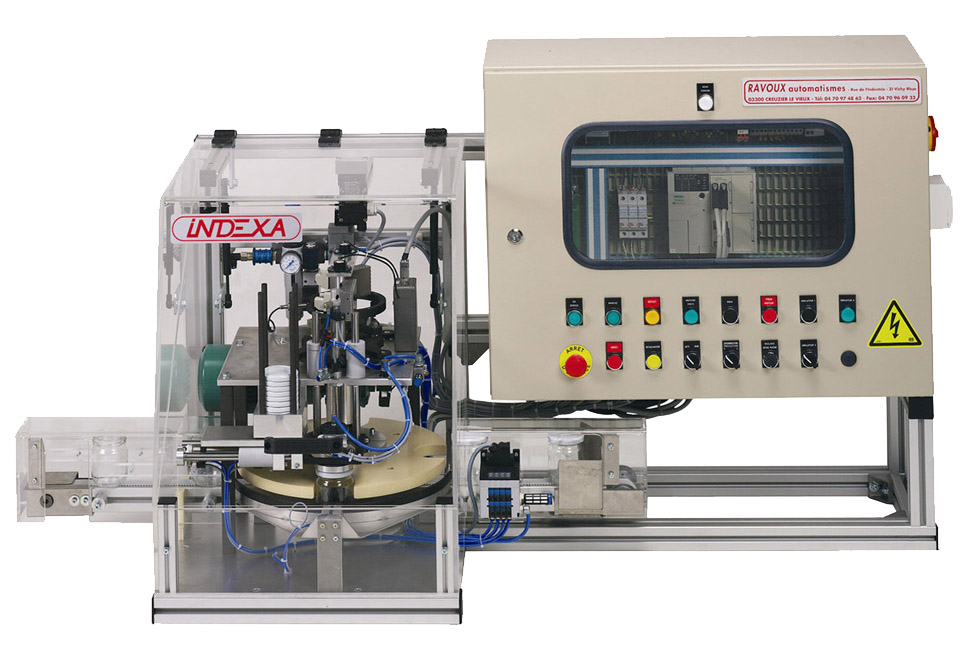
\includegraphics[width=0.9\linewidth]{img/Indexa.jpg}
   \caption{Système capsuleuse bocaux}
   \label{img1}
  \end{minipage}
\end{figure}

Ce système comprend plusieurs parties (cf figure \ref{img2}) : 
\begin{itemize}
 \item un convoyeur linéaire d'alimentation des bocaux, 
 \item un système électromécanique de transfert et d'indexation des bocaux (motoréducteur, mécanisme à Croix de Malte, étoile de transfert), 
 \item un magasin de stockage des capsules, 
 \item une partie opérative pneumatique de pose et de vissage des capsules (vérin V1, tête de vissage comprenant les vérins V2 et VR, ventouse et vacuostat). Le vacuostat est une cellule permettant d'assurer la mise en dépression de la ventouse afin d'effectuer la préhension de la capsule. 
 \item un vérin de serrage des bocaux sous la tête de vissage, 
 \item un convoyeur linéaire d'évacuation des bocaux, 
 \item une partie commande par automate programmable TSX17 et un pupitre de commande. 
\end{itemize}

\begin{figure}
  \centering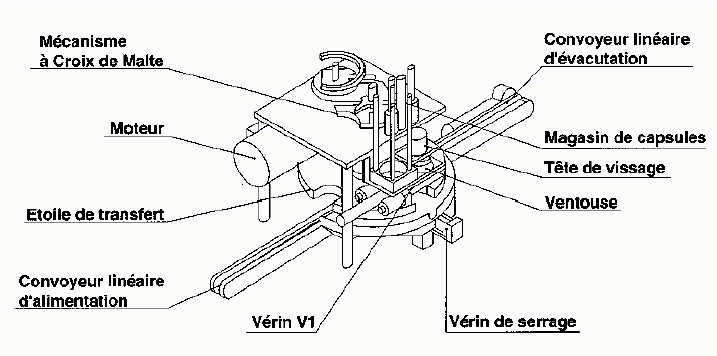
\includegraphics[width=0.9\linewidth]{img/Global_indexa.png}
    \caption{les composants du système}
  \label{img2}
\end{figure}

La dépose et le vissage d'une capsule sont assurées par : 
\begin{itemize}
 \item trois vérins pneumatiques, deux vérins linéaires \textbf{V1} et \textbf{V2} et un vérin rotatif \textbf{VR}. Le vérin rotatif \textbf{VR} est solidaire de la tige du vérin \textbf{V2} dans le mouvement de translation de celle-ci,
 \item une ventouse fixée sur le vérin rotatif et reliée à un vacuostat.
\end{itemize}


Sur la figure \ref{img2} et sur les schéma en perspective des figure \ref{img3} et \ref{img4}, les vérins \textbf{V2} et \textbf{VR} sont intégrés dans la tête de vissage. Le vérin de serrage n'est pas représenté sur la photographie de la figure \ref{img2}. 

Dès qu'un bocal est présent sous la tête vissage, il est bloqué par le vérin de serrage. Le lancement du cycle de dépose et de vissage est conditionné par la présence d'un bocal, notée bp, et par le retour de tous les actionneurs à leur position initiale. Le cycle se déroule de la façon suivante : la tige du vérin \textbf{V1} pousse une capsule située dans le magasin de capsules sous la tête de vissage.

La position du capteur de fin de course «tige sortie» est notée v11. 
\begin{itemize}
 \item \textbf{V2} descend et entraîne dans son mouvement \textbf{VR} sur lequel est fixée la ventouse. La position du capteur de fin de course \og tige sortie \fg de \textbf{V2} est déterminée par l'arrivée de la ventouse sur la capsule et est notée \textbf{v211}. 
 \item \textbf{V2} remonte et entraîne dans son mouvement \textbf{VR} qui a saisi la capsule au moyen de la ventouse. La position du capteur \og tige rentrée \fg est notée \textbf{v20}. 
 \item \textbf{V1} recule, libérant la place sous la tête de vissage, et se repositionne sous le magasin de capsules. La position du capteur \og tige rentrée \fg est notée \textbf{v10}.
 \item \textbf{V2} descend, en entraînant \textbf{VR}, afin de déposer la capsule sur le bocal. La position du capteur \og tige sortie \fg est notée \textbf{v212}. 
 \item \textbf{VR} visse la capsule sur le bocal. La position du capteur \textbf{vr1} du vérin rotatif ne doit pas être atteinte avant la fin d'une temporisation lancée en même temps que le mouvement de rotation du vérin \textbf{VR} (fin de temporisation notée \textbf{tpvr}). 
 \item dès que la dépression au niveau de la ventouse est supprimée le bocal est débloqué et \textbf{V2} remonte en entraînant \textbf{VR} qui tourne alors en sens inverse. L'arrêt de ce mouvement de rotation est donné par un capteur \textbf{vr0}
\end{itemize}

\begin{figure}
  \centering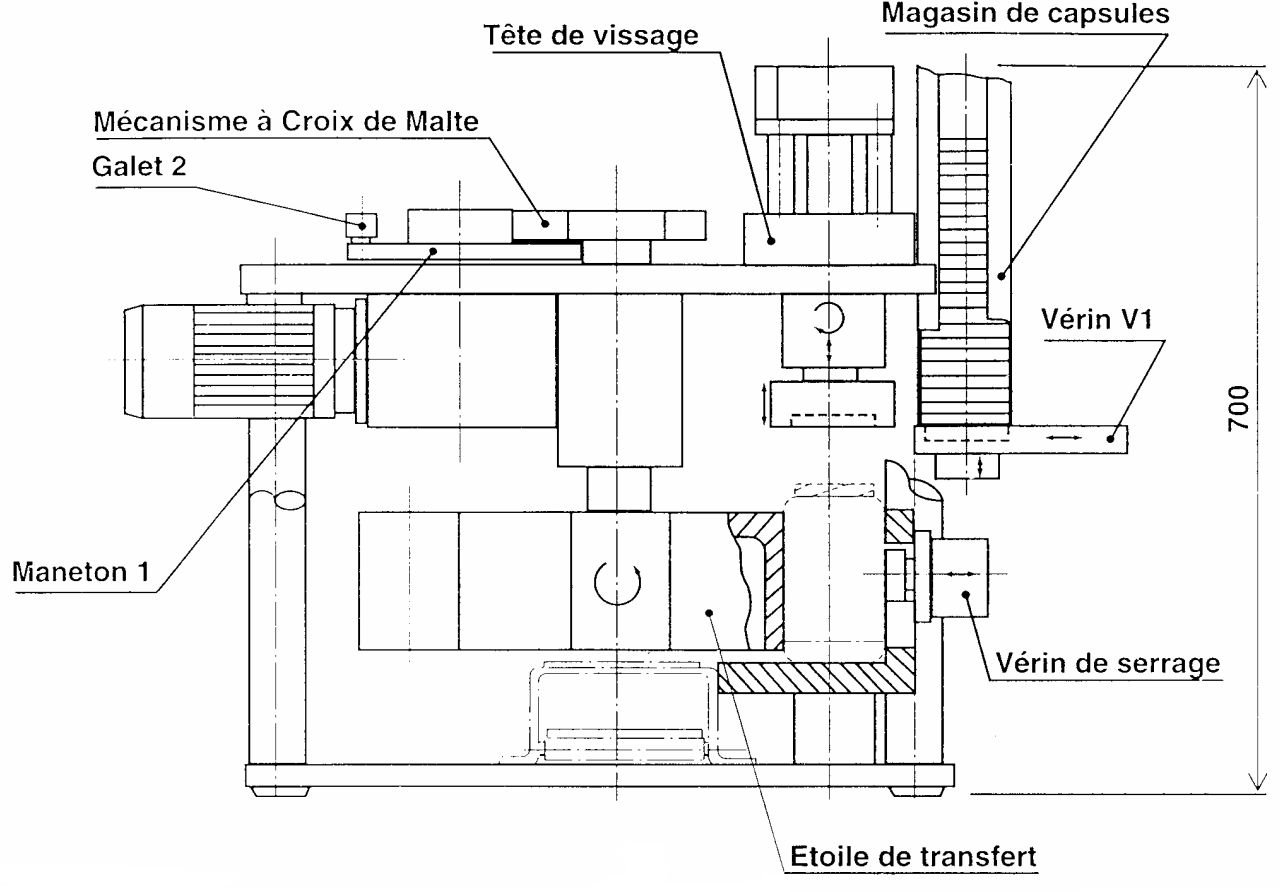
\includegraphics[width=0.8\linewidth]{img/Indexa1.png}
    \caption{Vue partielle}
  \label{img3}
\end{figure}

\begin{figure}
  \centering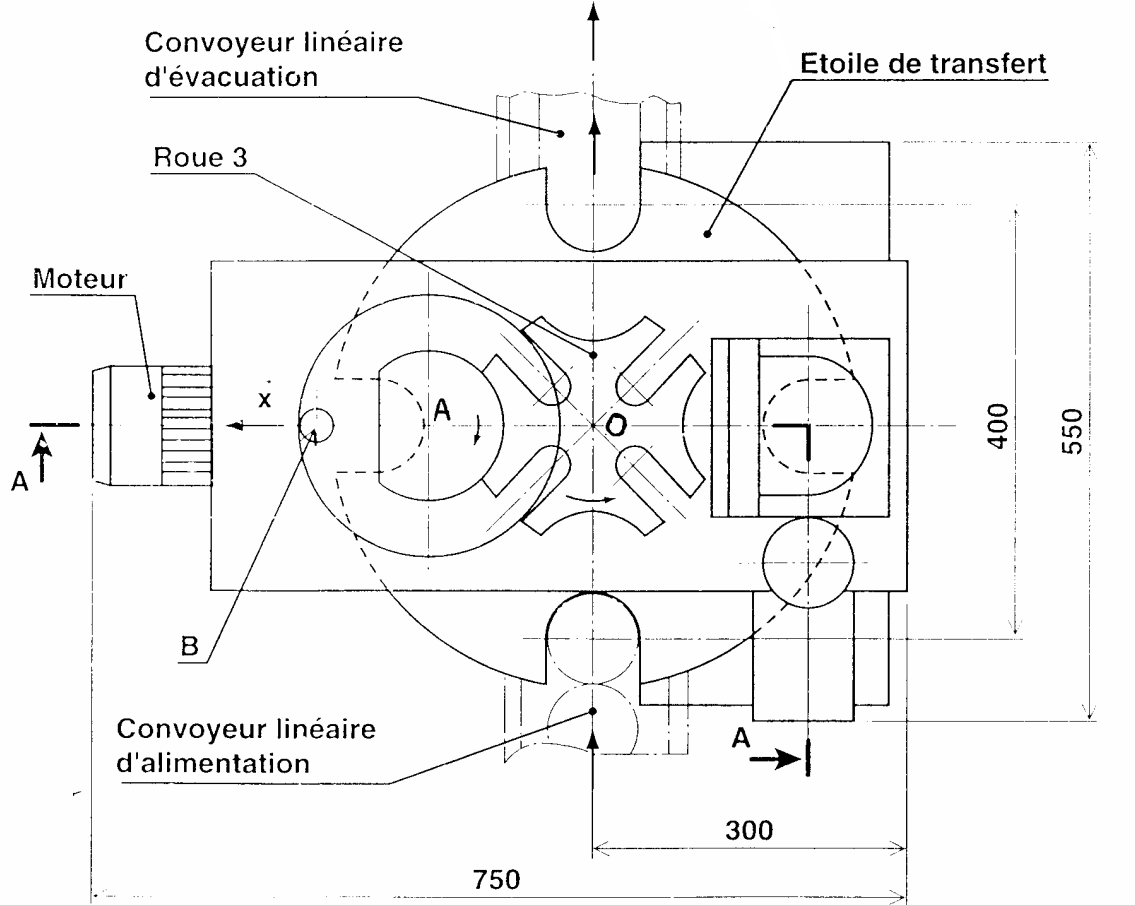
\includegraphics[width=0.7\linewidth]{img/Indexa2.png}
    \caption{Système croix de Malte}
  \label{img4}
\end{figure}

%\subsection{Encapsulation}
%
%\begin{minipage}{0.15\linewidth}
% 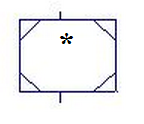
\includegraphics[width=0.7\linewidth]{img/Encapsulation1.png}
%\end{minipage}
% \hfill
%\begin{minipage}{0.8\linewidth}
%Étape encapsulante : Cette notation indique que cette étape contient d'autres étapes dites encapsulées. 
%\end{minipage}
%
%\vspace{1cm}
%
%\begin{minipage}{0.15\linewidth}
% 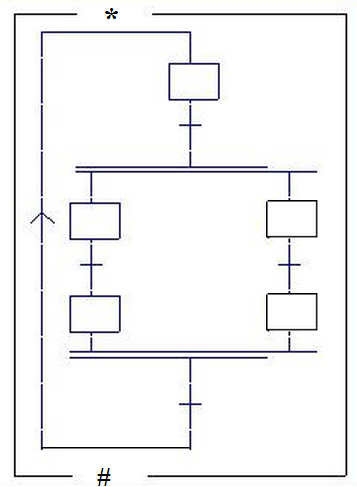
\includegraphics[width=1\linewidth]{img/Encapsulation2.png}
%\end{minipage}
% \hfill
%\begin{minipage}{0.8\linewidth}
%Représentation graphique d'une encapsulation : Une encapsulation $\sharp$ d'une étape encapsulante $*$ peut être représentée par le grafcet partiel des étapes encapsulées.
%\end{minipage}
%
%\vspace{1cm}
%
%\begin{minipage}{0.15\linewidth}
%{\Large $X*/G\sharp$}
%\end{minipage}
% \hfill
%\begin{minipage}{0.8\linewidth}
%Désignation globale d'une encapsulation : Une encapsulation $\sharp$ d'une étape encapsulante $*$.
%\end{minipage}

\paragraph{Question 1:} A partir de vos observations sur le système, compléter le diagramme suivant. Choisir la sortie du vérin V1 afin de bloquer le bocal comme première étape.

\begin{center}
 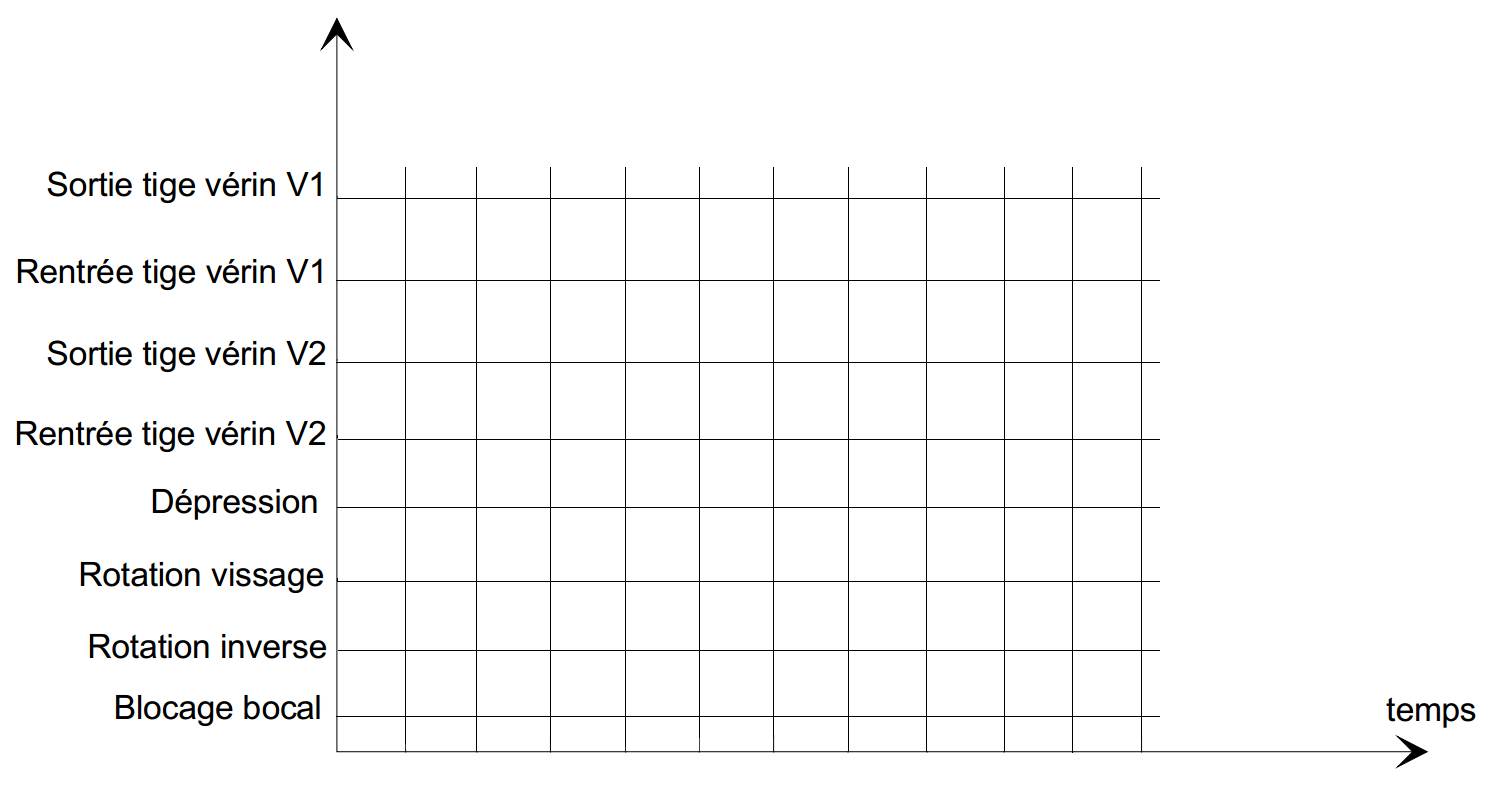
\includegraphics[width=0.7\linewidth]{img/Chronogramme.png}
\end{center}

\paragraph{Question 2:}

À partir de ce chronogramme, compléter le diagramme décrivant le fonctionnement séquentiel du poste de dépose et de vissage des capsules. On supposera qu'à l'état initial du diagramme, la partie opérative est correctement configurée, et qu'en particulier tous les vérins sont en position \og tige rentrée \fg. L'initialisation de la partie opérative n'est pas demandée dans ce diagramme.

\begin{center}
 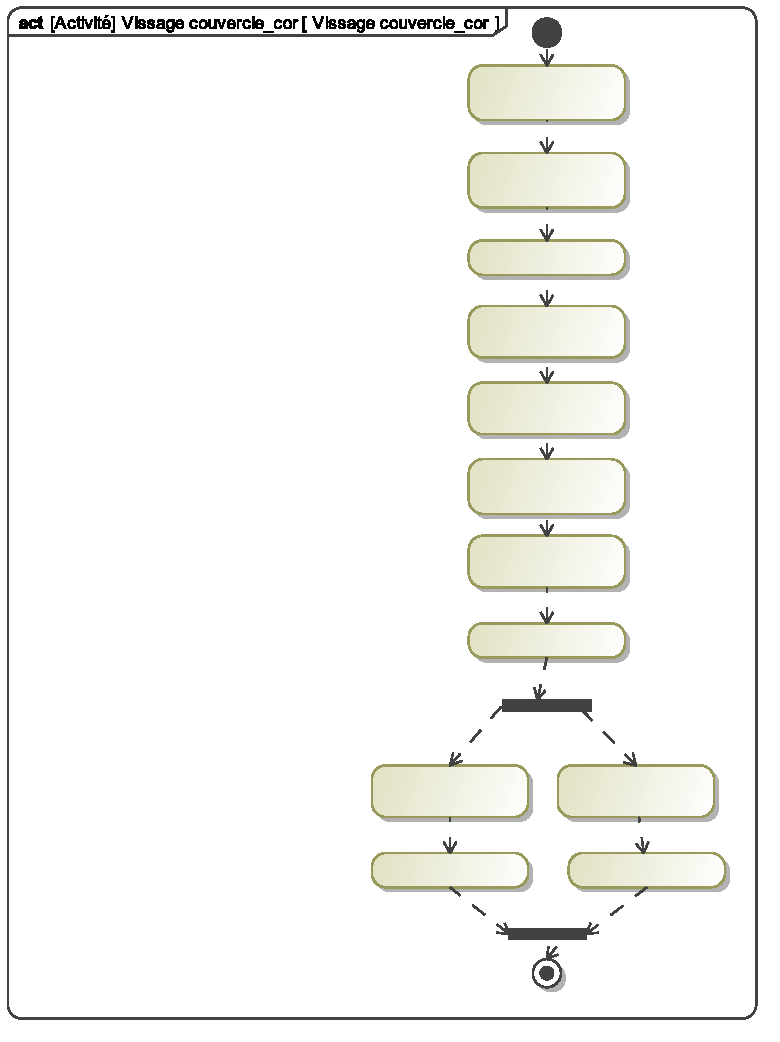
\includegraphics[width=\linewidth]{img/Vissage_couvercle}
\end{center}

Cette première solution demandée n'attend aucune structure évoluée de hiérarchisation. 

\newpage

\paragraph{Question 3:} Pour chaque étape et chaque transition, déterminer le capteur utilisé.

\reponse[10]

\end{document}
